143. \begin{figure}[ht!]
\center{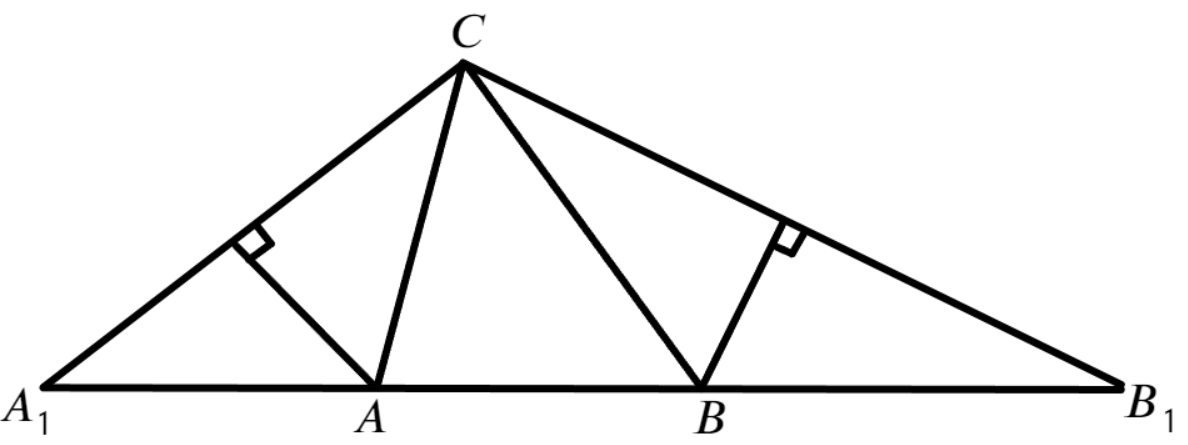
\includegraphics[scale=0.35]{g7-142.png}}
\end{figure}\\
Предположим, что треугольник $ABC$ построен. На продолжении отрезка $AB$ за точку $B$ отложим отрезок $BB_1,$ равный $BC,$ а на продолжении отрезка $AB$ за точку $A$ --- отрезок $AA_1,$ равный $AC.$ Треугольники $A_1AC$ и $B_1BC$ --- равнобедренные. Поэтому  $\angle A_1 = \cfrac{1}{2} \angle A,\  \angle B_1 = \cfrac{1}{2} \angle B,\ A_1B_1 = A_1A + AB + BB_1 = AC + AB + BC = P.$ Треугольник, равный треугольнику $A_1B_1C,$ строим по стороне (равной $P)$ и двум прилежащим к ней углам
$(\angle A_1 = \cfrac{1}{2}\angle A,\ \angle B_1 =\cfrac{1}{2}\angle B).$  Серединные перпендикуляры к сторонам $A_1C$ и $B_1C$ пересекают отрезок $A_1B_1$ в искомых вершинах $A$ и $B.$\\
